\documentclass[aps,twocolumn,secnumarabic,nobalancelastpage,amsmath,amssymb,
nofootinbib]{revtex4-1}
% \documentclass[12pt,letterpaper,oneside]{report}

\usepackage{graphics}      % standard graphics specifications
\usepackage{graphicx}      % alternative graphics specifications
\usepackage{longtable}     % helps with long table options
\usepackage{url}               % for on-line citations
\usepackage{bm}  
%\usepackage{dblfloatfix}
\usepackage[explicit]{titlesec}
\titlespacing\section{0pt}{8pt}{4pt}
% \usepackage{amsmath}
% \usepackage{amsfonts}
% \usepackage{mathtools}
% \usepackage{amssymb}
% \usepackage{latexsym}
% \usepackage{fancyhdr}
% \usepackage{gensymb}
% \usepackage{dsfont}
% \usepackage{hyperref}
% \usepackage{changepage}
% \setlength{\headheight}{15pt}
% \setlength{\textwidth}{6.5in}
% \setlength{\oddsidemargin}{0in}
% \setlength{\evensidemargin}{0in}
% \setlength{\topmargin}{0in}
% \pagestyle{fancy}
% \lhead{Peter Weck} \chead{Permutation entropy analysis of dynamical turbulence} \rhead{June 24, 2014}

\setlength{\parskip}{5pt}
\begin{document}
\title{Permutation Entropy Analysis of Dynamical Turbulence in an  \\MHD Plasma Wind Tunnel and the Solar Wind}
\author{P.J. Weck, D.A. Schaffner, R.T. Wicks, and M.R. Brown}
\affiliation{Swarthmore College, Swarthmore, PA 19081}
\begin{abstract}
The permutation entropy of Bandt and Pompe and the Jensen-Shannon statistical complexity are used to analyze turbulence in the MHD plasma wind tunnel of the Swarthmore Spheromak Experiment. MHD wind-tunnel turbulence is compared to turbulence data from the solar wind and the Large Plasma Device using these metrics, and it is found that the wind-tunnel configuration exhibits more truly turbulent dynamics than LAPD but less turbulent dynamics those in the solar wind. 
\end{abstract}
\maketitle

\section{Introduction}
Since Bandt and Pompe introduced their probability distribution based on ordinal patterns in arbitrary time series in 2002 \cite{bandt2002}, their methodology has found a wide variety of applications, from tracking the effects of anesthetic drugs on the brain \cite{li2010,jordan2008,olofsen2008} to informing economic policy \cite{bariviera2013,zunino2010,zunino2011}, among many others \cite{kowalski2007,soriano2011,saco2010,suyal2012,sun2010}. In 2007, Rosso \textit{et al} applied the ordinal pattern distribution of Bandt and Pompe to a time series analysis using the complexity-entropy plane, or “CH plane”, capable of differentiating between periodic, chaotic, and stochastic systems \cite{rosso2007}. The CH plane has been used to determine the statistical character of fluctuations in several physical systems, including magnetic flux ropes \cite{gekelman2014} and electron heat transport \cite{maggs2013} in magnetized plasmas. However, to our knowledge the approach has yet to be extended to the study of dynamical plasma turbulence, either in the solar wind or in a dynamical laboratory plasma source. The purpose of the present paper is to fill this gap in the understanding of the CH-character of plasma systems, and provide one further point of comparison between the MHD wind tunnel configuration and the solar wind.

We compare the CH positions of MHD wind tunnel, solar wind, and drift-wave plasmas, as well as model chaotic systems and stochastic processes, and find that although more stochastic than the drift-wave plasma source and comparable in entropy and complexity to known stochastic proccesses, MHD wind tunnel data is both less entropic and more complex than the solar wind. This suggests that further steps must be taken before the wind tunnel configuration can generate the fully developed turbulence seen in the solar wind data. Both larger confinement volumes and longer lifetimes are potential avenues for improving the correspondance between  solar wind and MHD wind tunnel positions on the CH plane.

The MHD wind tunnel configuration of the Swarthmore Spheromak Experiment (SSX) consists of a plasma gun which fires a spheromak of magnetized plasma into an $\sim1$ meter long cylindrical copper flux conserver, as described in \cite{zhang2011} and \cite{schaffner2014}. Probes embedded in the chamber collect data on turbulent fluctuations in $\dot{B}$ as the plasma evolves down the length of the tube, eventually relaxing into a Taylor state \cite{gray2013}. After injection the plasma is completely dynamical, as there is no guide or vacuum field in the body of the chamber. By varying the amount of magnetic flux through the core of the gun, or "stuffing flux", between 0.0 and 1.5 mWb, the magnetic helicity of the injected plasma can be finely controlled, as described in \cite{schaffner2014}. Magnetic helicity corresponds to the degree of twistedness in the magnetic field, so varying injected helicity affects the resulting turbulent dynamics of the plasma as it evolves towards a relaxed Taylor state. In our CH plane analysis of turbulence in the SSX plasma source, $\dot{B}$ time series for a variety of injected helicities were used. 

 Multi-day magnetic fluctuation records from both fast and slow solar wind streams measured by the \textit{Wind} spacecraft were selected for comparison. Fast streams are characterized by high velocities, low densities, and  few large-scale structures while slow streams are slower, denser, and more slightly more structured. \textit{Wind} is positioned near 1 AU, and is equipped to collect high cadence (3 s) magnetic field vector data.   The magnetic vector component antiparallel to the direction of mean field (away from the sun) was used in our analyses. Magnetic fluctuations are on the order of $10$ nT in both the fast and slow stream signals. 

%\vspace{6mm}

\section{Permutation Entropy and the CH Plane}
The permutation entropy and thereby the CH plane position of an arbitrary time series is defined in terms of a window length called the embedding dimension $n$. The embedding dimension determines the size of patterns investigated in calculating the entropy and complexity of the series. The instances of each ordinal patterns of that size are counted in order to assoiciate an ordinal pattern probability distribution with the time series, from which the calculation of entropy and complexity is straightforward.

For embedding dimension $n$, the probability distribution introduced by Bandt and Pompe consists of the frequencies of occurrence of all possible length $n$ ordinal patterns in segments of $n$ consecutive terms from an arbitrary time series \cite{bandt2002}. In their methodology, a length $n$ ordinal pattern is defined for a segment $s = ( x_t,x_{t+1},\ldots,x_{t+(n-1)} )$ of the time series as the permutation $\pi$ of the index set $\{0,1,\ldots,n-1 \}$ corresponding to the ranking of the $x_i$ in ascending order, namely $x_{\pi_t}< x_{\pi_{t+1}}<\ldots< x_{\pi_{t+(n-1)}}$. In order to guaruntee a unique result, if $x_i = x_j$ where $i<j$, then in the ranking $x_i <x_j$. For example, if $x_0 = 5$,  $x_1= -2$,  and $x_2 = 0.33$ are three consecutive terms in the time series, then since $x_1 < x_2 < x_0$, the ordinal pattern for this segment is the permutation $\pi = (1,2,0)$.  Given a time series of length $L$, the corresponding ordinal pattern probability distribution $P= \{p(\pi) \}$ is defined in terms of all $L-n+1$ length $n$ segments $s$ in the series and all $n!$ permutations $\pi$ of order $n$ by
\begin{align}
p(\pi) = \frac{|\{s: \text{$s$ has ordinal pattern $\pi$}\}| }{L-n+1}. 
\end{align}
where $|\ldots|$ denotes cardinality. The permutation entropy $PE$ is defined as Shannon's information entropy for this ordinal pattern probability distribution, or
\begin{align}
PE  = -\sum^{n!} p(\pi) \log p(\pi)
\end{align}
where the $\log$ is base two.

Instead of considering consecutive points in calculating the ordinal pattern probability distribution for a time series, an embedding delay $\tau$ can be used to sample ordinal patterns on a larger time scale, thereby placing a lower limit on the size of structures investigated in the frequency sectra and focusing the analysis on a particular temporal scale. Embedding delays can be implemented as a simple sub-sampling of data in which only $L/\tau$ values of the time series are considered, as in \cite{maggs2013} and \cite{gekelman2014}, or all $\tau$ of these portions of the original time series can be used as in \cite{bandt2005}, henceforth referred to as the length-preserving method. For example, for an embedding delay $\tau=10$ using the first method, a new time series $X'$ of length $L'=\frac{1}{10}L$ is generated by selecting every tenth value of the original series $X$ and the ordinal pattern probability distribution calculated for that series in the usual manner. In the  length-preserving method, segments $ ( x_t,x_{t+10},\ldots,x_{t+10(n-1)} ) $ of $X$ are used to calculare the ordinal pattern probability distribution, where $t$ runs from $1$ to $L-10(n-1)$, thereby including the $9/10$ths of the dataset thrown out in the first method. Which method is used depends in part on the length of the record in question. Unless  $L' \gg n!$, the first method may not yield reliable statistics \cite{gekelman2014}, and the length-preserving method thus appears preferable.


While the permutation entropy quantifies the randomness in an arbitrary time series, to quantify the degree of correlational structure a measure of statistical complexity such as the Jensen-Shannon complexity is required \cite{rosso2007}. The Jensen-Shannon complexity, or $C_{JS}$, is a functional of the discrete distribution $P$ of $N$ probabilities associated with the time series. Once normalized such that $0 \leq C_{JS} \leq 1$, 
\begin{align}
C_{js}[P] = -2\frac{S \left[ \frac{P+P_e}{2} \right] - \frac{1}{2}S[P]-\frac{1}{2}S[P_e] }{\frac{N+1}{N} \log(N+1)-2 \log(2N)+\log(N)}H[P]
\end{align}
Where $S$ is the Shannon entropy, $H$ is the normalized Shannon entropy $S/S_{\text{max}}$, and $P_e=\{\frac{1}{N}, \ldots, \frac{1}{N} \}$ is the uniform distribution. When analyzing time series using the CH plane methodology of Rosso \textit{et al}, this measure of statistical complexity is evaluated by associating with the time series the ordinal pattern probability distribution of Bandt and Pompe, so that $N=n!$, $S[P]=PE$ and $H[P]=PE_{\text{norm}}=PE/\log(n!)$. The statistical nature of time series is then evaluated by comparing their positions on the CH plane, $PE_{\text{norm}} \times C_{JS}$.

In interpreting the CH position of experimental data, it is often useful to compare them to model  stochastic processes and chaotic systems. To illustrate the regions of the plane corresponding to paradigmatically stochastic and chaotic dynamics, stochastic fractional Brownian motion (fBm) and chaotic Henon, skew tent, and logistic maps are included in the $n=5$ CH plane shown in Figure 1. The range of fBm points displayed was generated by varying the corresponding Hurst exponent between 0 and 1, thereby scanning the degree of correlation between succsessive increments of motion from strong negative correlations to positive correlations. Also shown in Figure 1 are curves demarcating the minimum and maximum complexity bounds of the CH plane. The nature of the dependence of $C_{JS}$ on $H$ constrains the possible values of the former as a function of the latter to fall between these curves, as described in \cite{lopez1995} and \cite{calbet2001}.
\begin{figure*}[!htbp]
\centerline{
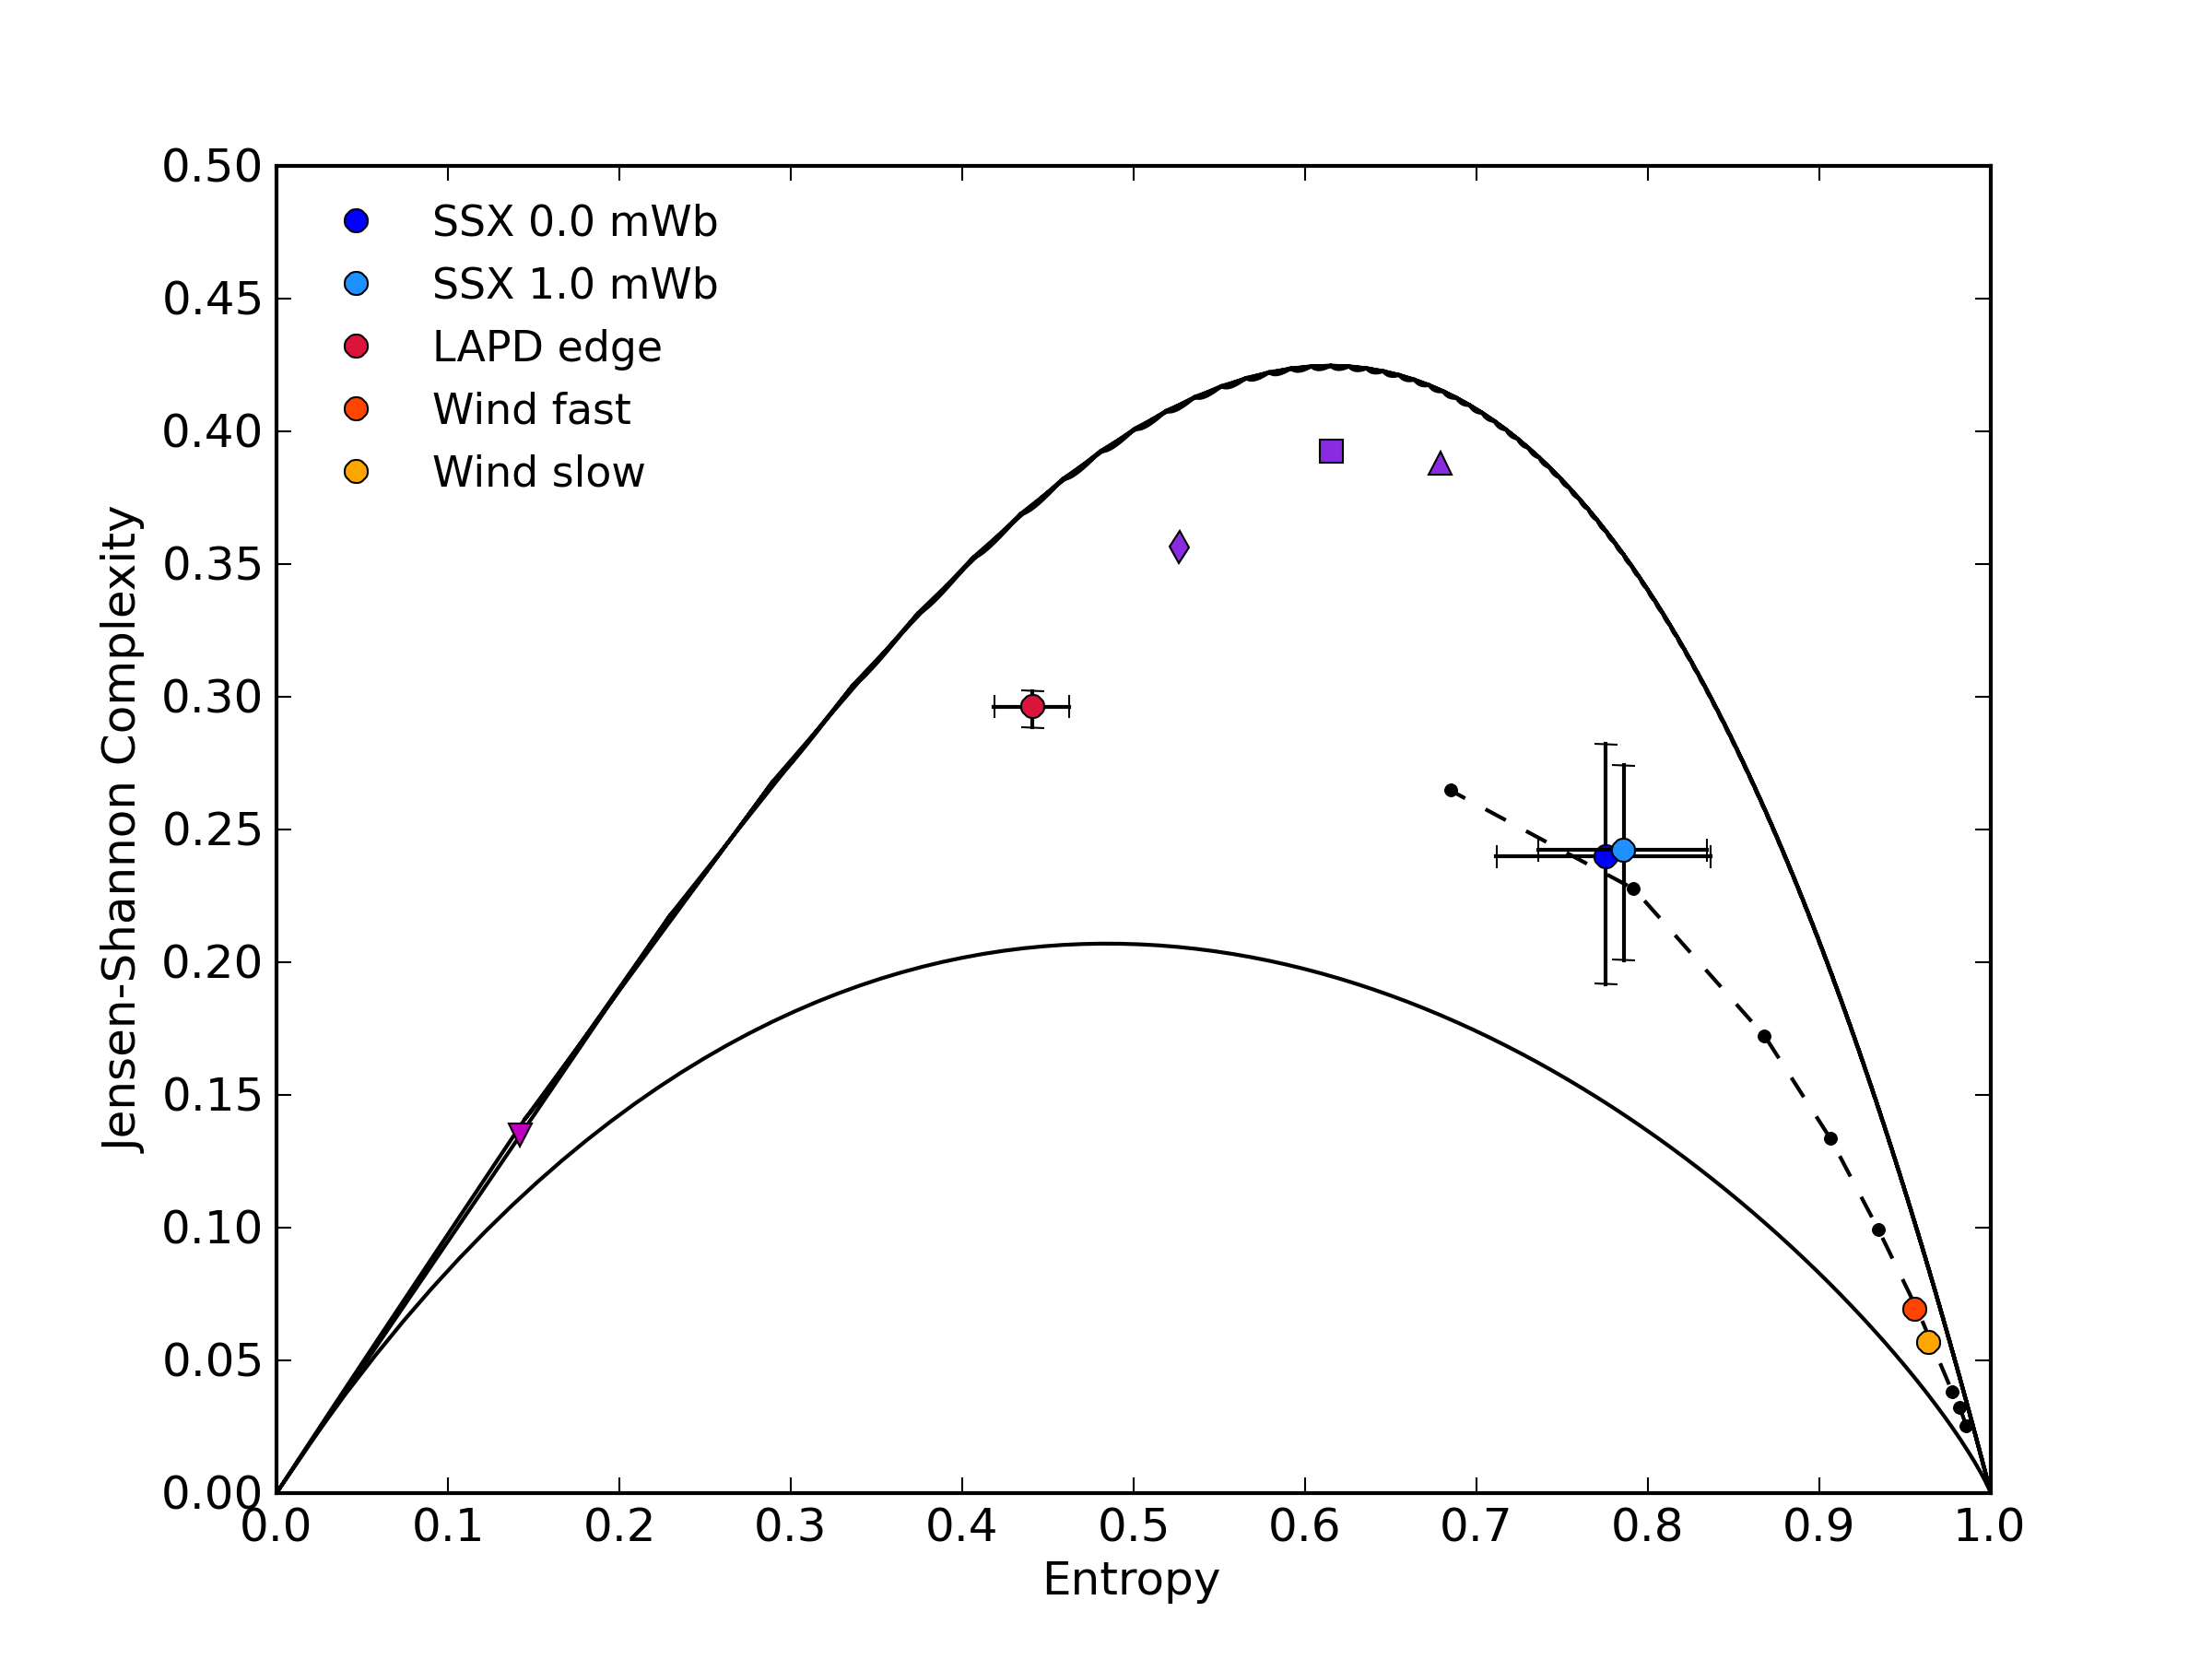
\includegraphics[width=17cm]{fig1.png}}
\caption{\label{Figure 1} The $n=5$ CH plane  with SSX $\dot{B}$ data for two injected helicities in blue, \textit{Wind} fast and slow stream $B$ data in orange, chaotic LAPD edge plasma ion saturation current signals in red, and paradigmatic chaotic systems and stochastic processes for comparison. Crescent shaped curves show the maximum and minimum possible $C_{JS}$ for a given $PE_{\text{norm}}$.}
\end{figure*}

\section{CH comparison of SSX and WIND data}
The $\dot{B}$ fluctuation signals used in our CH plane analysis of SSX data  were recorded by a 16-channel, 3-direction, single-loop pickup coil probe embedded in the midplane of the cylindrical wind tunnel, with a $65$ MHz sampling rate and 14 bit dynamic range. $20$ $\mu$s windows were used in our analysis, corresponding to 1,300-value time series. Approximately $40$ shots were taken at each of $8$ stuffing fluxes between $0.0$ and $1.5$ mWb, corresponding to injected helicities ranging from $0$ to $7 \times 10^{-5}$ Wb$^2$ \cite{schaffner2014}. In this manner, over $15,000$ magnetic fluctuation time series were generated, over a range of radial positions, directions, injected helicities, and shots. The normailized permutation entropy and Jensen-Shannon comlexity were calculated for each series, using $n=5$ in order to satisfy the common condition $L > 5n!$, as recommended in \cite{amigo2008} and \cite{riedl2013}. The length-preserving embedding delay method was employed to preserve this condition after filtering. Each series was analysed from $40-60~\mu$s after discharge, as the turbulence signals exhibit a stationary phase during that period. SSX mangetic field fluctuation spectra resolve structures well only up to $9$ or $10$ MHz, so an embedding delay of $\tau=8$ was used to limit the range of frequencies investigated. The average position of series from all three directions of the inner 4 probe coils at each of two helicity settings is shown in blue in Figure 1. Error bars indicate standard deviations above and below the mean.  

\begin{figure}[!htbp]
\centerline{
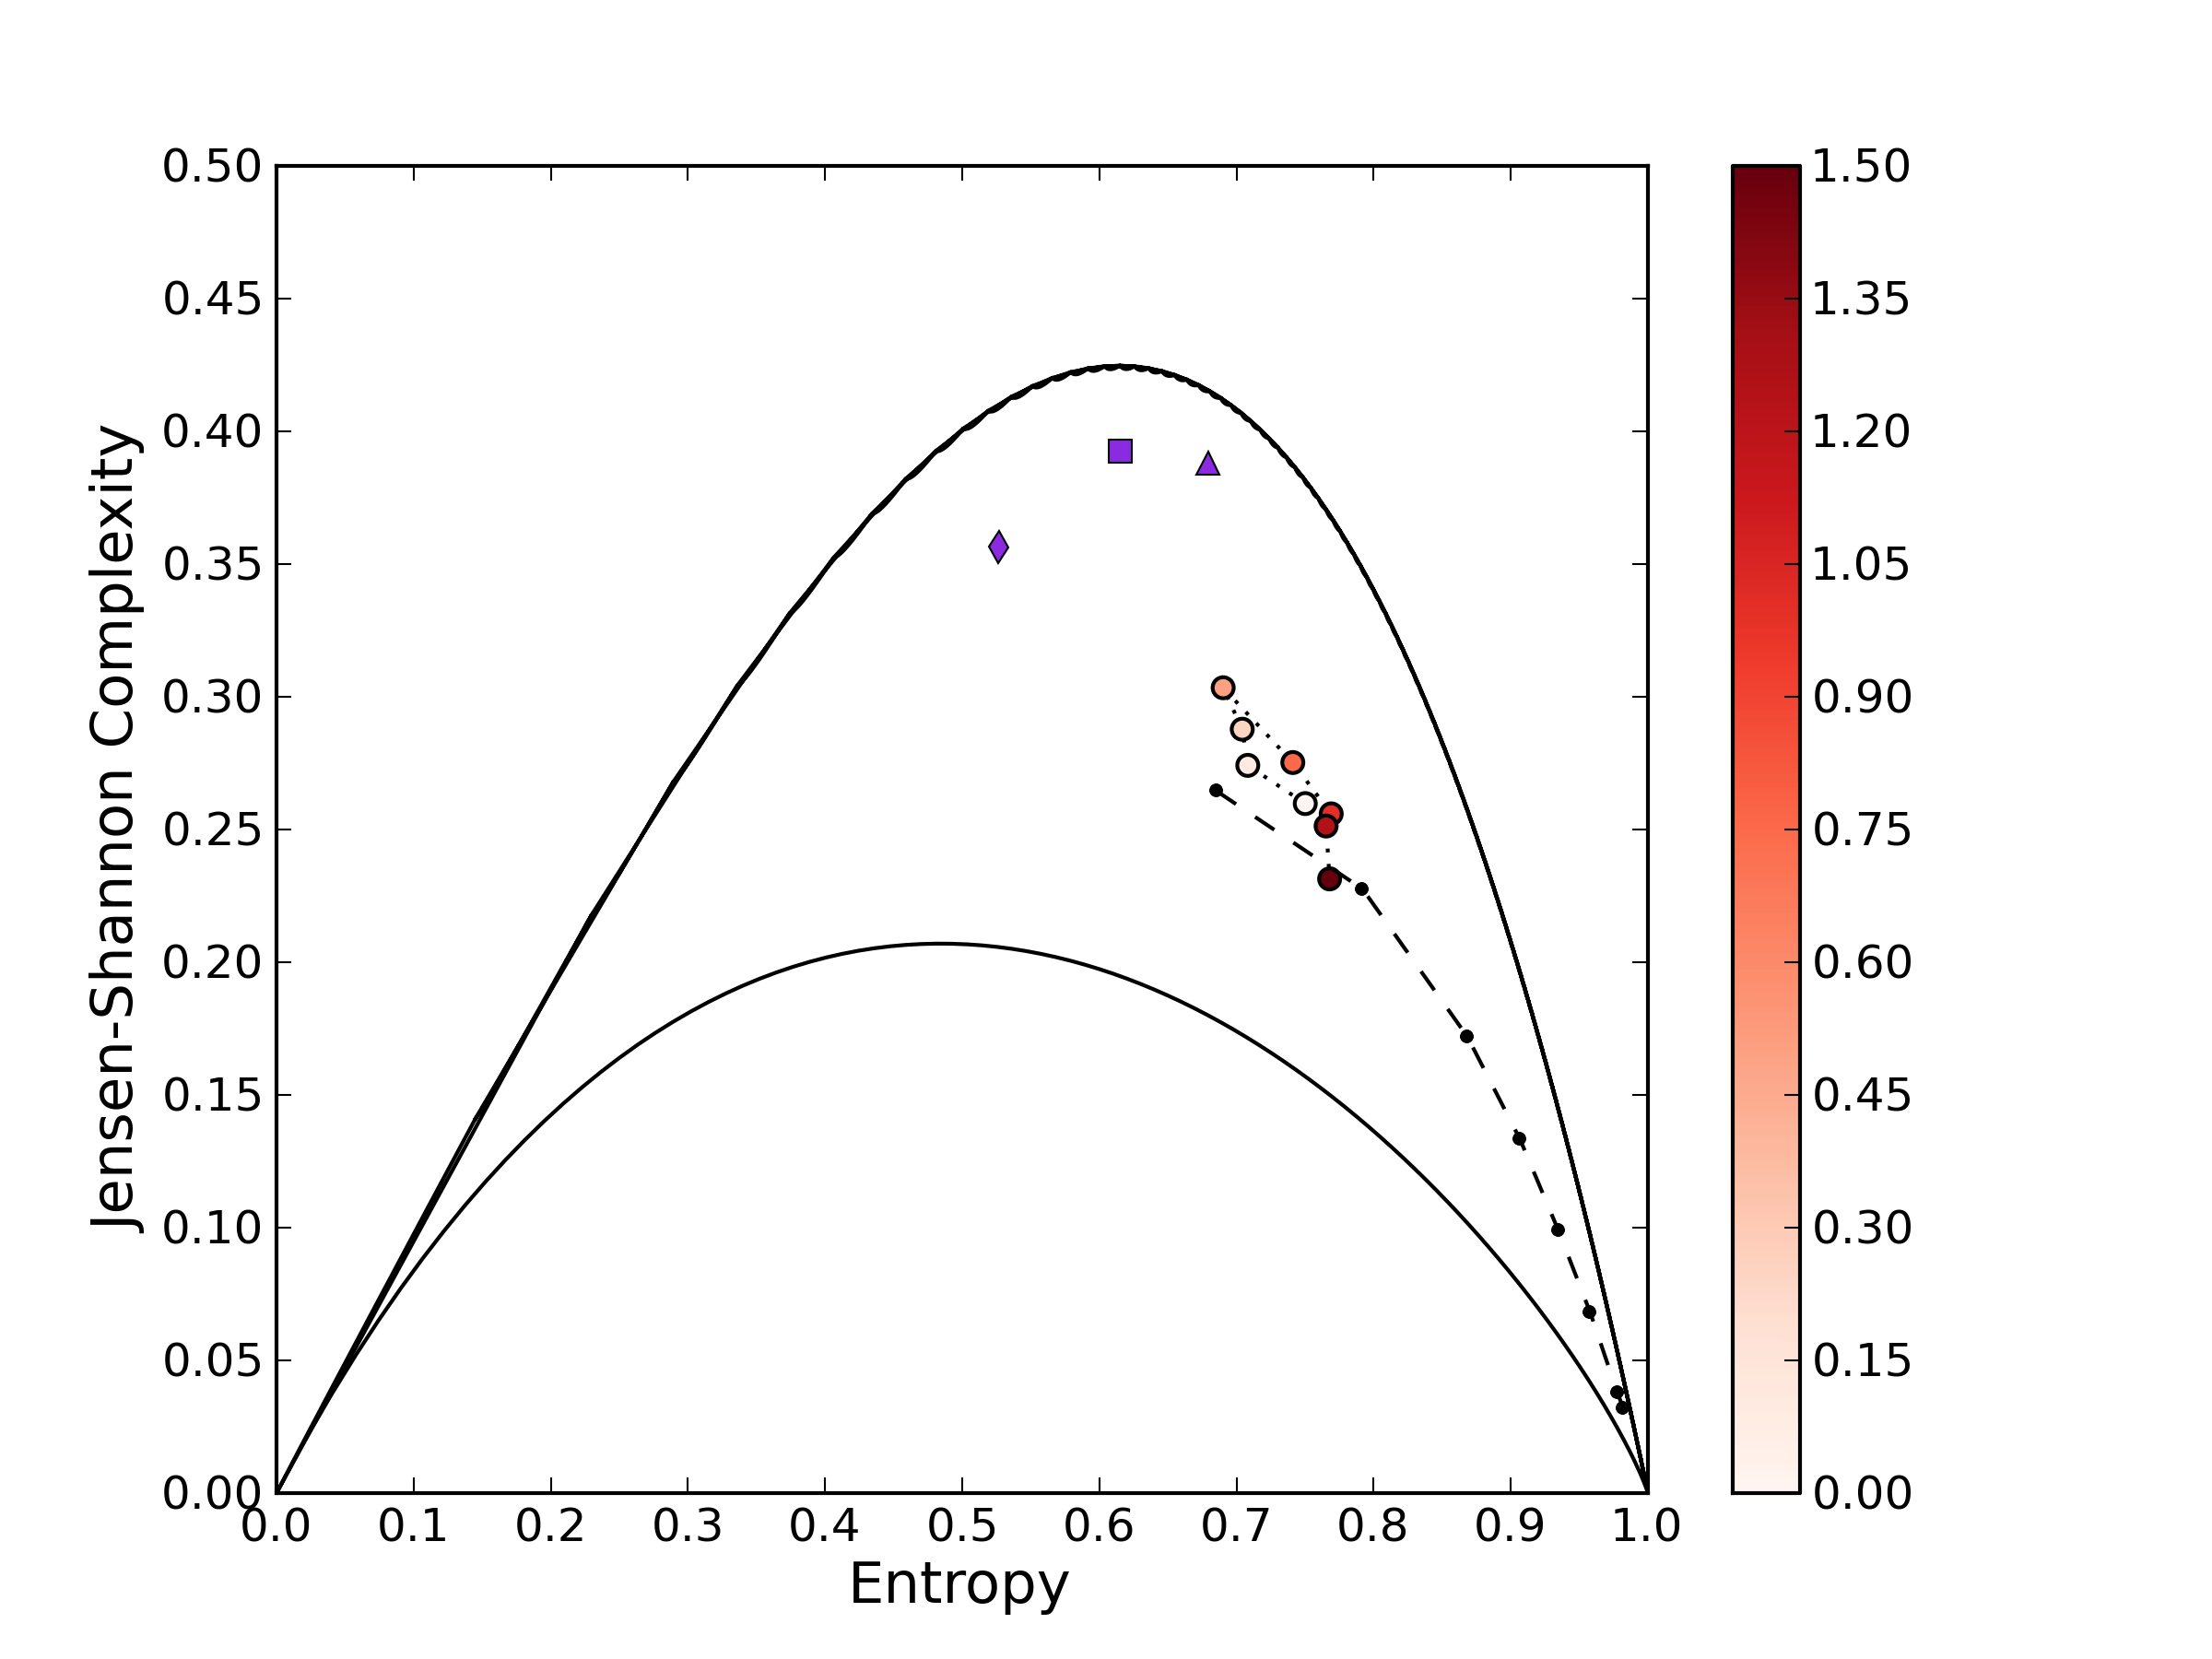
\includegraphics[width=8.5cm]{fig2.png}}
\caption{\label{Figure 2} The color scale represents stuffing flux, in mWb. Dotted lines connect succsessive helicity settings to illustrate the trend. Data was acquired from the tip of the 16 channel probe.}
\end{figure}

Figure 1 also shows the positions of both fast and slow stream magnetic flustuations in the solar wind.  The fast stream magnetic signal from \textit{Wind} consisted of almost 230,000 values, and the slow stream signal of over 170,000. Since both signals were highly stationary, a set of subseries could be treated as an ensemble. The length of subseries was chosen in conjunction with the embedding delay so as to satisfy the condition $L_{wind}/\tau_{wind} = L_{ssx}/\tau_{ssx}$ while maximizing differentiation between the Jensen-Shannon complexities of the fast and slow streams and keeping the number of subseries on the order of $10$. Based on these criteria, entropies and complexities were averaged over $20$ subseries each $11,375$ values in length for the fast stream signal and $15$ subseries of the same length for the slow stream. Delays of $70$ were used, which limits the  upper frequency range of the dynamics under investigation to well within the intertial range. Error bars are not displayed due to the small size of deviations in complexity and entropy from the mean.

Previous work using frequency spectra has suggested that the edge fluctuations of magnetized plasmas in the Large Plasma Device (LAPD) and other devices are chaotic, rather than stochastic in nature \cite{maggs2012}. For purposes of comparison, the permutation entropy and Jensen-Shannon complexity were also calculated for $1.5$ MHz ion saturation current signals from a radial position corresponding to edge plasmas in the LAPD.  The CH position of the LAPD edge plasma shown in Figure 1 in red was averaged over $25$ shots and $5$ sections of $1000$ values for each shot with no embedding delay. 

\begin{figure}[!htbp]
\centerline{
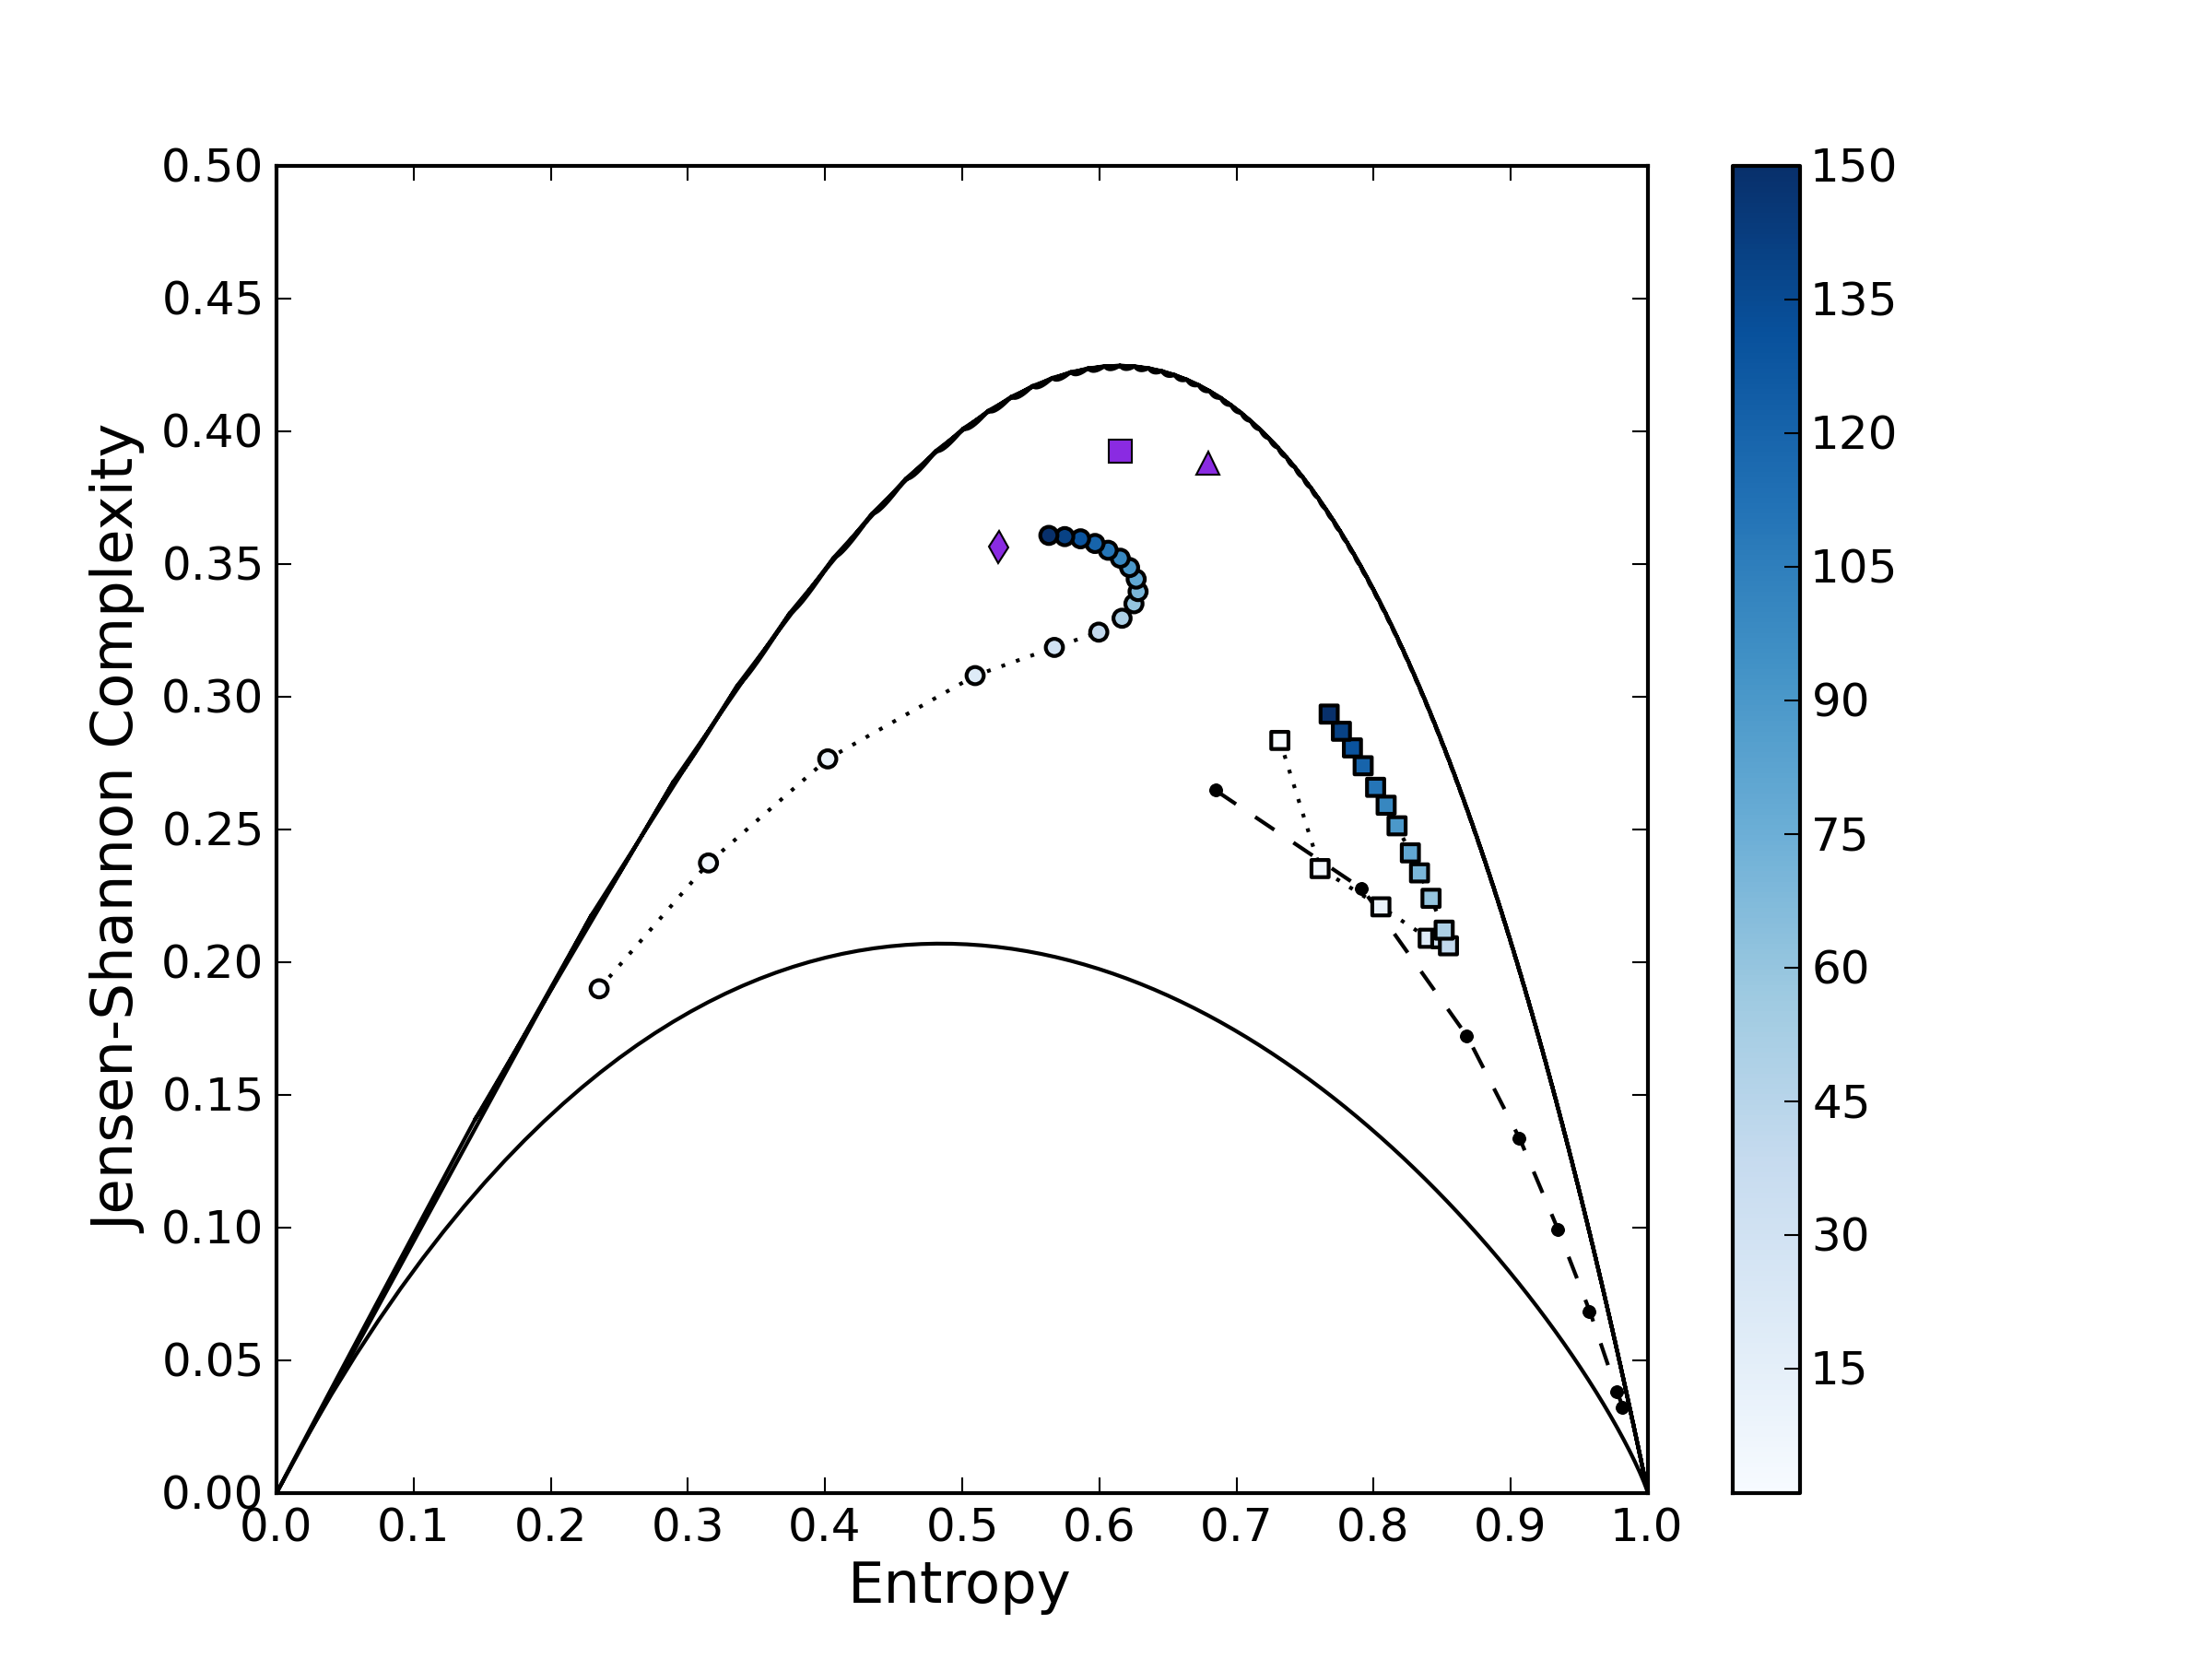
\includegraphics[width=8.5cm]{fig3.png}}
\caption{\label{Figure 3}Trajectories of SSX $B$ and $\dot{B}$ data as function of embedding delay from $1$ to $150$, color-coded by increasingly dark shades of blue. }
\end{figure} 

As expected, the LAPD edge plasma signals analyzed occupy the central region of the plane which has previously been associated with more chaotic than stochastic dynamics in experimental data \cite{maggs2013, gekelman2014}. The SSX turbulence data at the $0.0$ mWb (left-hand blue marker) and $1.0$ mWb (right-hand marker) stuffing flux settings, on the other hand, occupy a higher entropy range comparable to fractional brownian motion with positive correlation between successive increments of motion. The proximity of SSX $\dot{B}$ signals to stochastic processes like fBm suggest that these signals are dominated by stochastic rather than chaotic dynamics. Furthermore, the relative  positions of SSX and LAPD sources on the $PE_{\text{norm}} \times C_{JS}$ plane indicate that the SSX plasma source is more truly turbulent than the LAPD edge plasma. 

According to these metrics, magnetic fluctuations in the solar wind near $1$ AU more random than either wind tunnel MHD turbulence or even classical Brownian motion (fBm with Hurst exponent of $1/2$).  The fast stream signal (lower orange circle) exhibits slightly more entropy and less complexity, supporting identification of faster streams with more stochastic dynamics.  Although it has been well documented that the solar wind exhibits well-developed turbulence (cite), this is the first time that developed MHD turbulence in an astrophysical plasma has been identified based on a complexity-entropy analysis or compared in this manner to other plasma sources.

Although little spread was observed in either the \textit{Wind} or LAPD data analyzed, significant spread was seen in the complexity and entropy of SSX $\dot{B}$ signals. Perhaps the most interesting contribution to this spread was from injected helicity.  Figure 2 shows the helicity dependence of SSX $\dot{B}$ data, plotting CH positions for signals over a scan of stuffing fluxes measured at the innermost channel of the probe, averaged over directions and shots. The same ordinal pattern paramters used to generate Figure 1 ($n=5$ and $\tau=8$) were used in Figure 2. There is a clear increasing trend in complexity up to $0.5$ mWb, after which the complexity decreases with stuffing flux. As a result the data executes a tight "loop" in the plane extending up just past $C_{JS}=0.3$ with entropies between $0.68$ and $0.78$. Thus the degree of "twistedness" in the injected spheromak has consequences for the degree of correlational structure in the the resulting relaxation dynamics.

In some cases, additional information can be gained about the underlying dynamics of a system by examining the permutation entropy and Jensen-Shannon complexity as functions of the embedding delay $\tau$ \cite{zunino2012}. Figure 3 compares SSX $\dot{B}$ signals averaged over all shots, directions, and inner four probe channels to the corresponding $B$ signals obtained by integrating $\dot{B}$ for a scan of the embedding delay from $\tau=1$ to $\tau=150$ ($\tau=1$, $5$, and then $10$, $20$, etc. in steps of $10$). As before, the length-preserving method was employed. However, despite the use of the length preserving method, useful statistics seem only to be obtainable for our 1300 value series up to $\tau \approx 50$. For larger embedding dimensions, the number of length $n$ segments used in calculating the ordinal pattern distribution is reduced by over 15%. The poorly "filled out" PDF manifests itself in artificially high complexities; note the abrupt hook shapes executed by the trajectories of both $B$ and $\dot{B}$ data near $\tau=50$. 

\section{Conclusion}
In this paper, fully dynamical laboratory and astrophysical plasmas have been studied using the ordinal pattern-based CH plane introduced by Rosso \textit{et al} for the first time. Comparing the relative positions of drift-wave, MHD wind tunnel, and solar wind plasmas, it was found that the three systems occupy different regions of the CH plane, suggesting that despite the broad-band spectra exhibited by all these systems, the CH analysis is capable of clearly differentiating between drift-wave, partially developed, and fully developed turbulence. Considering that drift-wave turbulence is thought to be a result of the nonlinear interactions of relatively few modes while fully developed turbulence contains too many modes to distinguish, it would appear that the CH positions of these magnetized plasmas are reflective of the number of degrees of freedom of the system in question. In particular, the smaller number of modes generating drift-wave turbulence in LAPD edge plasmas may be reflected by the low-middle entropy and middle-range complexity of that system, while high entropy and low complexity of magnetic fluctuations in the solar wind may reflect the multitude of degrees of freedom active in that system. Based on the relative CH positions of SSX MHD wind tunnel and $\textit{Wind}$ data, although SSX is on its way towards the highly stochastic turbulence in the solar wind, this analysis indicates that further steps are needed for SSX  to most accurately model solar wind turbulence. The confined nature of the experiment and short lifetimes involved are both potential contributors to the discrepancy in CH positions. After all, besides the boundary conditions imposed by atrophysical bodies, the solar wind is an unconfined and extremely long lived plasma. Which if any of these two parameters could be varied to reduce complexity and increase entropy of SSX  to that of the solar wind is an open question. In any case, the CH methodology has provided us with one more means of comparison and a clear goal to work towards.



\bibliography{master}
\bibliographystyle{plain}
\nocite{*}
\end{document}
